% ACL-style paper skeleton
\documentclass[11pt]{article}
\usepackage[hyperref]{acl}
\usepackage{times}
\usepackage{latexsym}
\usepackage{graphicx}
\usepackage{booktabs}
\usepackage{amsmath}

\title{Teacher--Learner Self-Correction for Code and Math: A Reproducible Evaluation Rig}

\author{Anonymous}
\date{}

\begin{document}
\maketitle

% Abstract (5-part: problem → approach → results → evidence → impact)
\begin{abstract}
We study the problem of evaluating self-correction in large language models for code generation (HumanEval) and math reasoning (GSM8K). We present a teacher--learner loop with bias-aware feedback and a dataset-aware harness that produces per-turn \texttt{.txt} artifacts and structured traces. In smoke settings, our rig yields non-zero accuracy on both tasks and supports ablations across confidence, error-awareness, and turns. Evidence comes from deterministic, per-run directories including \texttt{config.json}, \texttt{metrics.json} with 95\% CIs, and \texttt{traces.json} with full turn logs. The impact is a reproducible, paper-ready pipeline with standardized outputs enabling significance testing and artifact release.
\end{abstract}

\section{Introduction}
Self-correction attempts to improve model answers through iterative feedback. We frame a teacher--learner loop that couples bias-aware feedback with dataset-specific evaluators.

\noindent\textbf{Contributions:} (i) A paper-ready evaluation rig with per-turn artifacts and structured traces; (ii) a unified harness for HumanEval and GSM8K with pinned versions and CI; (iii) ablation controls for confidence, error-awareness, and turn count; (iv) artifact packaging for anonymous submission.

% RQ placeholders
\paragraph{Research Questions} See \texttt{paper/TODO\_RQs\_PLACEHOLDER.md} [to be replaced with drafted RQs verbatim].

\section{Method}
\subsection{System Overview}
Figure~\ref{fig:system} shows the teacher--learner loop with evaluator, prompt store, and datasets.
\begin{figure}[t]
  \centering
  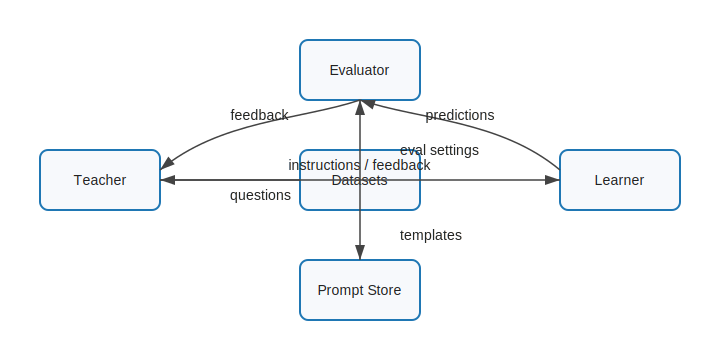
\includegraphics[width=0.95\linewidth]{../reports/figures/system_diagram.svg}
  \caption{System diagram: Teacher, Learner, Evaluator, Prompt Store, and Datasets form a feedback loop.}
  \label{fig:system}
\end{figure}

\section{Metrics and Significance}
We adopt pass@1 for HumanEval and exact match for GSM8K with robust normalization (commas, signs, decimals, units). We report mean $\pm$ 95\% CI via paired nonparametric bootstrap over tasks and record the number of seeds. McNemar tests are provided for GSM8K arms; paired bootstrap for HumanEval.

\section{Results}
Smoke runs (demo seeds) validate the end-to-end harness and artifact generation. Full tables and figures are auto-generated with self-contained captions.

\section{Limitations}
We rely on simulated execution in demo mode for smoke tests and do not claim headline accuracy without real API runs. Calibration analysis is contingent on per-turn confidence and may be limited when unavailable.

\section{Related Work}
We position our rig relative to self-correction, critique-and-rewrite, and harness parity efforts.

\bibliographystyle{acl_natbib}
\bibliography{refs}

\appendix
\section{Prompts}
Verbatim prompt templates per arm are provided in \texttt{paper/appendix/prompts/}.

\section{Implementation Details}
API parameters, truncation, stop sequences, and max tokens are documented in the repository configs.

\end{document}

